\chapter{Material adicional}
\label{chap:adicional}

\section {Análisis de resultados}

\subsection{Línea base - 5 clases}\label{analisis_bl_5}

En la figura \ref{distTassCine} se aprecia una gran diferencia en la distribución de clases, mostrando en las polaridades del conjunto de entrenamiento una tendencia de agrupación en torno a los extremos, mientras que en el conjunto de test se agrupan en torno a la neutralidad. 

\begin{figure}[H]
	\centering
	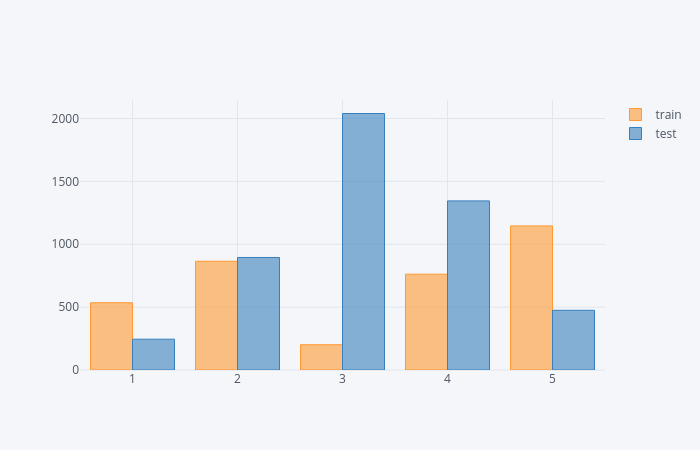
\includegraphics[width=1\textwidth]{imaxes/distCineTass.png}
	\caption{Distribución de polaridades en los conjuntos de entrenamiento y test.}
	\label{distTassCine}
\end{figure}

Este desbalanceo es una de las causas de los problemas de clasificación en distinto dominio, ya que el modelo tiende a clasificar los documentos con las polaridades que más destacan en el conjunto de entrenamiento, en este caso las clases con etiquetas 2 y 5, como se ve en la matriz de confusión representada en la figura \ref{conf5clases}.



\begin{figure}[H]
	\centering
	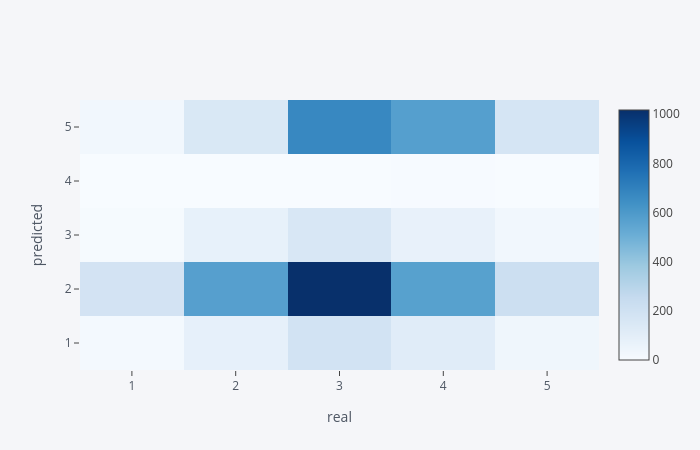
\includegraphics[width=1\textwidth]{imaxes/heatmap.png}
	\caption{Matriz de confusión de la clasificación en 5 clases.}
	\label{conf5clases}
\end{figure}


\section{Resultados GridSearch en Machine Learning}

\subsection{2 clases}

\begin{table}[H]
	\centering
	\begin{tabular}{|l|cccc|cccc|}
		\hline
		& \multicolumn{4}{c|}{CountVectorizer} & \multicolumn{4}{c|}{TF-IDF} \\
		\cline{2-9}
		&    acc &     f1 &    mse &  recall & acc &     f1 &    mse &  recall \\
		\hline
		lr      &  76.88 &  80.87 &  23.12 &   77.77 &  79.22 &  82.04 &  20.78 &   82.29 \\
		ls      &  76.60 &  80.52 &  23.40 &   77.85 &  80.99 &  \textbf{83.21} &  19.01 &   85.35 \\
		mb      &  79.93 &  \textbf{82.39} &  20.07 &   83.90 &  77.38 &  81.89 &  22.62 &   76.46 \\
		rf      &  73.55 &  77.10 &  26.45 &   77.44 &  70.92 &  74.85 &  29.08 &   75.12 \\
		\hline
	\end{tabular}
	\caption{Resultados en \% del mejor modelo obtenido en los k-folds}
	\label{result-cv-test}
\end{table}

\begin{table}[H]
	\centering
	\begin{tabular}{|l|cccc|cccc|}
		\hline
		& \multicolumn{4}{c|}{CountVectorizer} & \multicolumn{4}{c|}{TF-IDF} \\
		\cline{2-9}
		&    acc &     f1 &    mse &  recall & acc &     f1 &    mse &  recall \\
		\hline
		lr      &  63.44 &  \textbf{69.51} &  36.56 &   63.82 &  65.02 &  72.47 &  34.98 &   66.30 \\
		ls      &  62.55 &  65.74 &  37.45 &   65.66 &  64.56 &  73.09 &  35.44 &   64.97 \\
		mb      &  60.34 &  54.67 &  39.66 &   72.72 &  60.88 &  \textbf{73.29} &  39.12 &   60.41 \\
		rf      &  52.69 &  56.06 &  47.31 &   56.87 &  50.16 &  41.53 &  49.84 &   64.08 \\
		\hline
	\end{tabular}
	\caption{Resultados de la clasificación en el dominio de críticas de cine.}
	\label{result-cv-test-cine}
\end{table}

\subsection{3 clases}

\begin{table}[H]
	\centering
	\begin{tabular}{|l|cccc|cccc|}
		\hline
		& \multicolumn{4}{c|}{CountVectorizer} & \multicolumn{4}{c|}{TF-IDF} \\
		\cline{2-9}
		&    acc &     f1 &    mse &  recall & acc &     f1 &    mse &  recall \\
		\hline
		lr      &  67.86 &  67.86 &  105.59 &   67.86 &  74.32 &  74.32 &  80.37 &   74.32 \\
		ls      &  67.80 &  67.80 &  106.45 &   67.80 &  75.25 &  \textbf{75.25} &  76.65 &   75.25 \\
		mb      &  70.13 &  \textbf{70.13} &   96.74 &   70.13 &  71.86 &  71.86 &  90.22 &   71.86 \\
		rf      &  64.01 &  64.01 &  116.23 &   64.01 &  69.66 &  69.66 &  98.80 &   69.66 \\
		\hline
	\end{tabular}
	\caption{Resultados en \% del mejor modelo obtenido en los k-folds}
	\label{result-cv-test-3-clases}
\end{table}

\begin{table}[H]
	\centering
	\begin{tabular}{|l|cccc|cccc|}
		\hline
		& \multicolumn{4}{c|}{CountVectorizer} & \multicolumn{4}{c|}{TF-IDF} \\
		\cline{2-9}
		&    acc &     f1 &    mse &  recall & acc &     f1 &    mse &  recall \\
		\hline
		lr      &  39.74 &  \textbf{39.74} &  118.28 &   39.74 &  38.74 &  38.74 &  122.64 &   38.74\\
		ls      &  38.36 &  38.36 &  124.34 &   38.36 &  38.86 &  \textbf{38.86} &  122.16 &   38.86 \\
		mb      &  36.06 &  36.06 &  133.36 &   36.06 &  37.14 &  37.14 &  129.04 &   37.14 \\
		rf      &  34.94 &  34.94 &  119.24 &   34.94 &  34.42 &  34.42 &  139.92 &   34.42 \\
		\hline
	\end{tabular}
	\caption{Resultados de la clasificación en el dominio de críticas de cine.}
	\label{result-cv-test-3-clases-cine}
\end{table}

\subsection{5 clases}

\begin{table}[H]
	\centering
	\begin{tabular}{|l|cccc|cccc|}
		\hline
		& \multicolumn{4}{c|}{CountVectorizer} & \multicolumn{4}{c|}{TF-IDF} \\
		\cline{2-9}
		&    acc &     f1 &    mse &  recall & acc &     f1 &    mse &  recall \\
		\hline
		lr      &  41.05 &  41.05 &  268.06 &   41.05 &  45.58 &  45.58 &  222.82 &   45.58 \\
		ls      &  40.79 &  40.79 &  299.14 &   40.79 &  46.04 &  \textbf{46.04} &  214.90 &   46.04 \\
		mb      &  42.12 &  \textbf{42.12} &  257.29 &   42.12 &  42.38 &  42.38 &  285.56 &   42.38 \\
		rf      &  36.13 &  36.13 &  287.09 &   36.13 &  43.65 &  43.65 &  248.17 &   43.65 \\
		\hline
	\end{tabular}
	\caption{Resultados en \% del mejor modelo obtenido en los k-folds}
	\label{result-cv-test-5-clases}
\end{table}

\begin{table}[H]
	\centering
	\begin{tabular}{|l|cccc|cccc|}
		\hline
		& \multicolumn{4}{c|}{CountVectorizer} & \multicolumn{4}{c|}{TF-IDF} \\
		\cline{2-9}
		&    acc &     f1 &    mse &  recall & acc &     f1 &    mse &  recall \\
		\hline
		lr      &  14.08 &  14.08 &  373.52 &   14.08 &  13.54 &  13.54 &  360.28 &   13.54\\
		ls      &  12.44 &  12.44 &  384.74 &   12.44 &  12.70 &  12.70 &  376.00 &   12.70\\
		mb      &  18.52 &  18.52 &  267.64 &   18.52 &  11.56 &  11.56 &  390.06 &   11.56 \\
		rf      &  21.38 &  \textbf{21.38} &  257.68 &   21.38 &  15.26 &  \textbf{15.26} &  334.78 &   15.26 \\
		\hline
	\end{tabular}
	\caption{Resultados de la clasificación en el dominio de críticas de cine.}
	\label{result-cv-test-5-clases-cine}
\end{table}

\section{Trabajo futuro diseño web}

Con la intención de mejorar la UX/UI de la aplicación web, se plantea un rediseño enfocado a la minimalización y simplificación de la misma.

Se plantea el diseño entorno a 3 puntos:

\begin{description}
	\item [UX simple]: Un usuario debería saber que puede hacer en la aplicación de un vistazo. Una interfaz poco intuitiva puede suponer la frustración y por lo tanto pérdida de muchos usuarios.
	\item [Adaptarnos a la imagen de empresa]: Se deben seguir los estándares de diseño de la empresa cliente, véase: utilizar su logo, su paleta de colores, etc. Esto permitirá al cliente suavizar el impacto de la implantación de la herramienta en su ecosistema.
	\item [Enfocada en el producto]: Enfocar la interfaz al contenido importante, el producto.
\end{description}

\subsection{Página principal}

\begin{figure}[H]
	\centering
	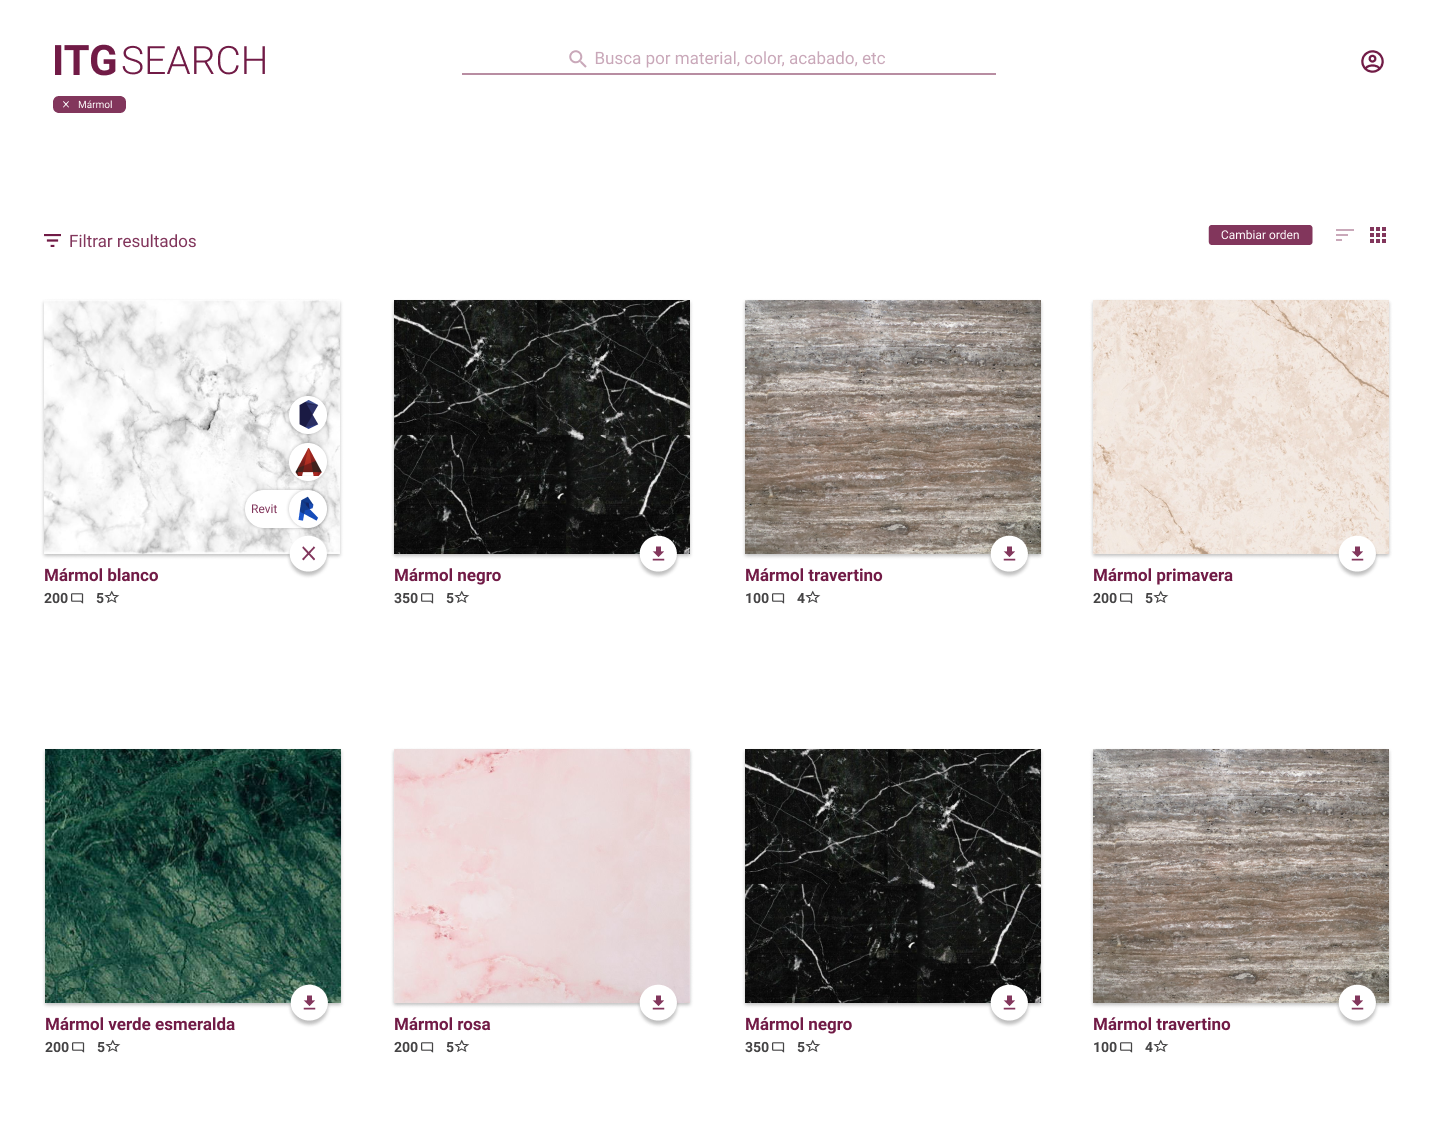
\includegraphics[width=1\textwidth]{imaxes/redHome.png}
	\caption{Página principal.}
	\label{redhome}
\end{figure}

Como vemos en la figura anterior hemos simplificado la interfaz y adoptado la paleta de colores de la empresa cliente.

A primera vista el usuario verá los artículos más destacados y toda la información relevante sobre los mimos, como número de comentarios, valoración y botón de descarga.

En este diseño asumimos el correcto funcionamiento del buscador, por lo que el usuario debería ser capaz de encontrar lo que desea entre los primeros 6 o 9 productos.

\subsection{Ficha de producto}

\begin{figure}[H]
	\centering
	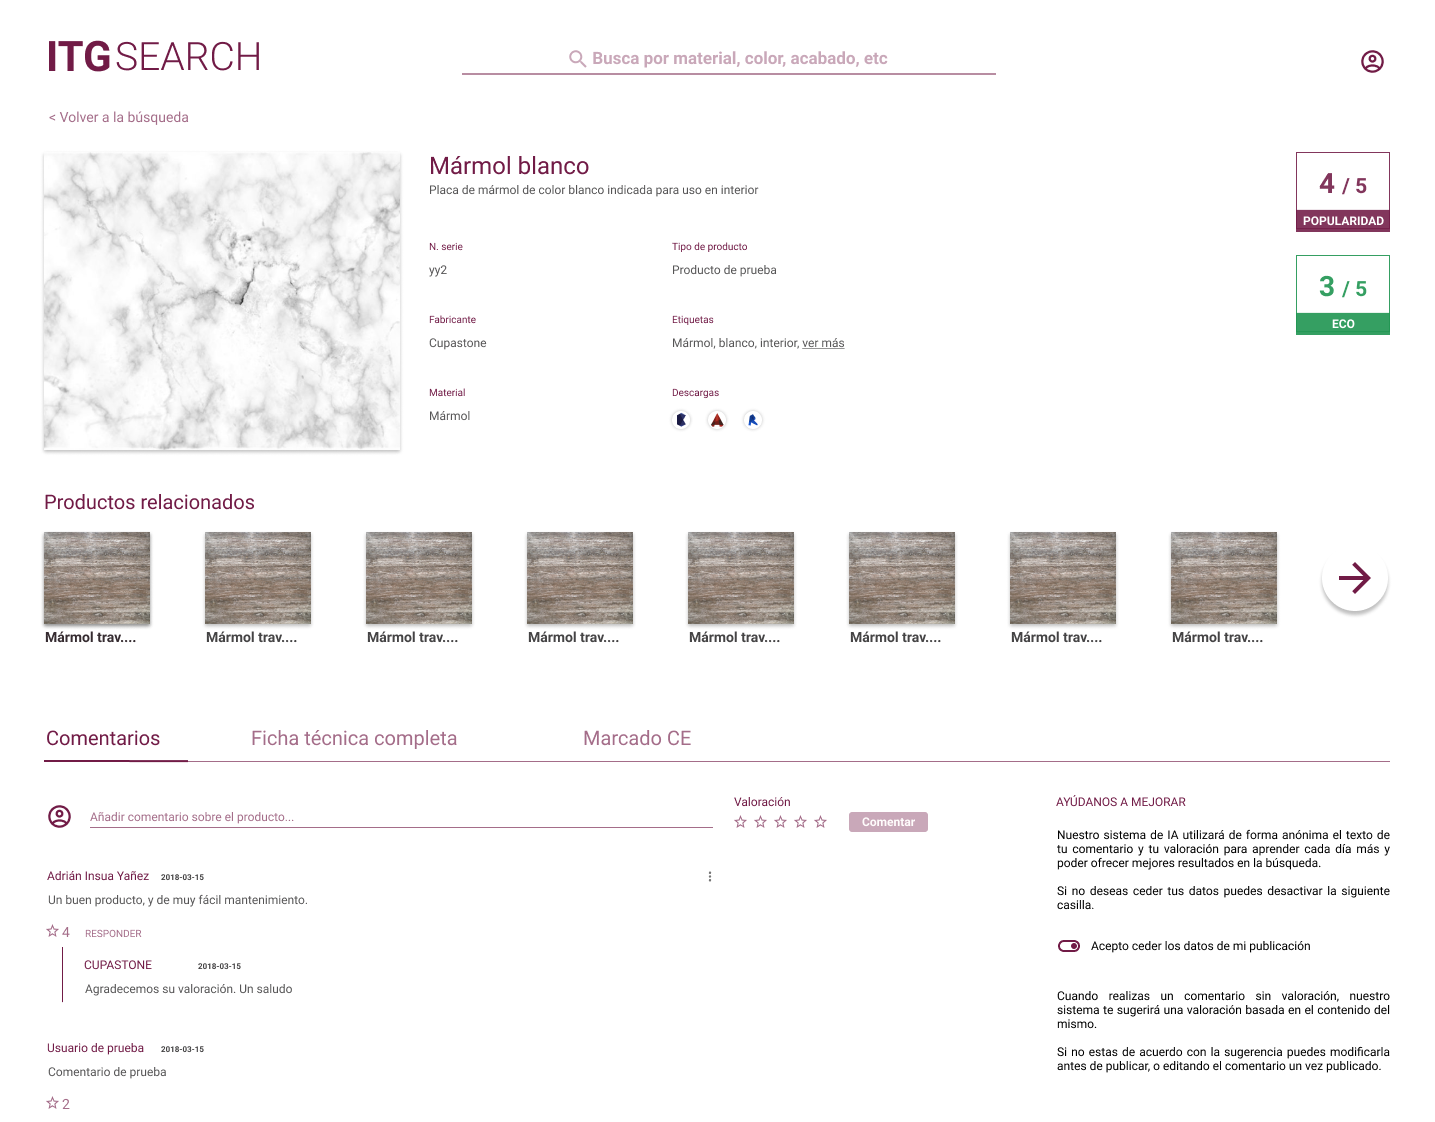
\includegraphics[width=1\textwidth]{imaxes/redProdDet.png}
	\caption{Ficha de producto.}
	\label{redProd}
\end{figure}

Para esta sección proponemos cambiar el modelo de ventana modal a una navegación completa, lo que nos permite introducir más información relevante sobre el artículo, sin que resulte molesto.

En esta ficha vemos además una sección de artículos relacionados, típica de las webs actuales, que se obtendrán a partir de las etiquetas del producto actual.

En la parte inferior se encuentra la sección de comentarios, y otras secciones secundarias. Hemos incluido el cuadro de inserción de comentarios y la nota sobre el uso de datos para mejorar el sistema de inteligencia artificial en la parte derecha de la sección de comentarios, evitando al usuario tener que dar pasos innecesarios.

